\section{Integration}
\label{sec:Int}
\subsection{Trapezoidal Rule}
We evaluate the integral for $f(x)$ in range $(a,b)$. One way would be to divide the range into $N$ slices like rectangles or trapezoids. As the name suggests, we approximate the function between $x_{i}$ and $x_{i+1}$ slices as a trapezium of $l1=f(x_{i})$ and $l2=f(x_{i+1})$ with separation  $h=(b-a)/N$, which will be same for all the trapeziums. Let the true value of the Integral be represented by $I$. Then the approximated integral is represented by $I_{0}$, given by:
\[\begin{split}
I_{0}&=\sum_{i=1}^{N}\dfrac{h}{2}[f(a+(i-1)h))+f(a+ih)] \\
%&=\dfrac{h}{2}[f(a)+f(a+h)+f(a+h)+......f(b)]
&=\dfrac{h}{2}[f(a)+f(b)+2(f(a+h))....2f(a+(N-1)h)]\\
&= \dfrac{h}{2}[f(a)+f(b)+2\sum_{i=1}^{N-1}f(a+ih)]\\
&\approx I\\
\end{split}
\]
Naturally, we will have greater precision for higher values of N. Generally, we use Adaptive Integral Method (discussed \hyperref[subsec:3.4]{here}), to obtain results within the desired level of accuracy.
\begin{lstlisting}[language=Python, caption=Trapezoidal Rule, frame=single, label={lst:L3} ]
def f(x):
	return x**4-2*x+1 #Function here
N= #Number Of Divisions
a= #start range
b= #end range
h=(b-a)/N
integ=f(a)/2+f(b)/2
for i in range(1,N):
	integ+=f(a+i*h)
integ*=h
print(integ) #Final Solution
\end{lstlisting}
\subsection{Simpson's Rule}
In Trapezoidal Rule, we approximate the curve by trapeziums, however we could fit a higher-order polynomial to our sliced function for better accuracy. Simpson's Rule does exactly that with polynomials of degree 2, i.e. Quadratic Expressions. We divide the range of $f(x)$, $(a,b)$ into $N$ equally spaced slices of width $h=(b-a)/N$. Let us consider 3 points, $\{-h,0,h\}$. The Quadratic polynomial passing through these points would be:
 
\[	f(x)=ax^{2}+bx+c\]
\[	f(-h)=ah^{2}-bh+c\]
\[	f(0)=c\]
\[	f(h)=ah^{2}+bh+c\]
Solving for the coefficients gives us the constants $a,b,c$ in terms of $h$. Now, we integrate over the slice $[-h,h]$ as follows:
\[\int_{-h}^{h}(ax^{2}+bx+c)dx=\dfrac{h}{3}[f(-h)+4f(0)+f(h)]  \]
Performing this integral for all slices of form $x_{i-1},x_{i},x_{i+1}$ returns the general approximate integral $I_{0}$ as:
\[\begin{split}
I_{0}&=\dfrac{h}{3}[f(a)+f(b)+4\sum_{k=1}^{Odd}f(a+kh)+2\sum_{k=2}^{Even}f(a+kh)]\\
&\approx I
\end{split}\]
Due to better order approximation, Simpson's rule generally yields more accurate results than the Trapezoidal rule in lesser steps ($N$). To obtain results within a specified degree of accuracy, we use the Adaptive Integral Method for Simpson's Rule (discussed \hyperref[subsec:3.4]{here}).
\begin{lstlisting}[language=Python, caption=Simpson's Rule, frame=single, label={lst:L4} ]
def f(x):
	return x**4-2*x+1 #function here
a= #start range
b= #end range
N= #Number of Divisions
h=(b-a)/N
s=f(a)+f(b)
for i in range(1,N,2):
	s+=4*f(a+i*h)
for i in range(2,N-1,2):
	s+=2*f(a+i*h)
s=s*h/3 
print(s)#Final Value
\end{lstlisting}
\subsubsection{Diffraction Limit Of Telescope}
Our ability to resolve detail in astronomical observations is
limited by the diffraction of light in our telescopes.  Light from stars
can be treated effectively as coming from a point source at infinity.  When
such light, with wavelength~$\lambda$, passes through the circular aperture
of a telescope (which we'll assume to have unit radius) and is focused by
the telescope in the focal plane, it produces not a single dot, but a
circular diffraction pattern consisting of central spot surrounded by a
series of concentric rings.  The intensity of the light in this diffraction
pattern is given by
\begin{displaymath}
I(r) = \biggl( {J_1(kr)\over kr} \biggr)^2,
\end{displaymath}
where $r$ is the distance in the focal plane from the center of the
diffraction pattern, $k=2\pi/\lambda$, and $J_1(x)$ is a Bessel function.
The Bessel functions~$J_m(x)$ are given by
\begin{displaymath}
J_m(x) = {\dfrac{1}{\pi}} \int_0^\pi \cos(m\theta - x\sin\theta) \ d\theta
\end{displaymath}
where $m$ is a nonnegative integer and $x\ge0$. \\

Here, I work out the image of the focal plane for light of $\lambda=500 nm$
\begin{lstlisting}[language=Python, caption=Bessel Function, frame=single, label={lst:L5} ]
def J(m,x):
	def f(t):
		return np.cos(m*t-x*np.sin(t))
	a=0
	b=np.pi
	N=1000
	h=(b-a)/N
	s=f(a)+f(b)
	for i in range(1,N,2):
		s+=4*f(a+i*h)
	for j in range(2,N-1,2):
		s+=2*f(a+j*h)
	s*=h/3
	return (1/(np.pi)*s)
\end{lstlisting}
\begin{figure}[H]
	\centering
	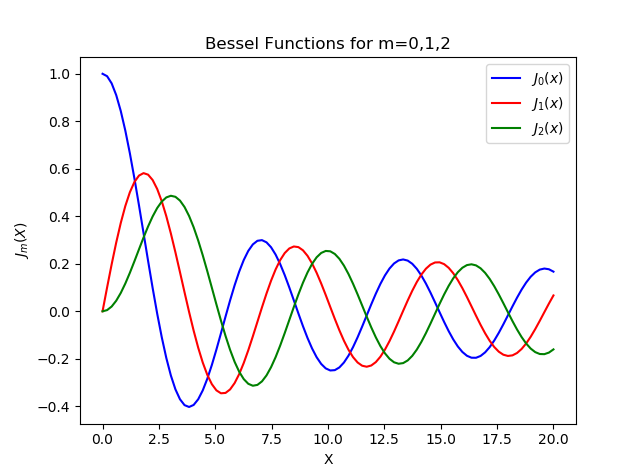
\includegraphics[width=0.7\linewidth]{BesselFunction}
	\caption{Plot of Bessel Functions}
	\label{fig:besselfunction}
\end{figure}

\begin{lstlisting}[language=Python, caption=Main Function, frame=single, label={lst:L6} ]
focal_plane=np.array([[0 for i in range(500)] for i in range(500)])
center=(250,250)
wavelength=62.5
k=2*np.pi/wavelength
def dist(point):
	x0,y0=center
	x,y=point
	return np.sqrt((x0-x)**2+(y0-y)**2)  
def I(r):
	return ((J(1,k*r))/(k*r))**2
for i in range(500):
	for j in range(500):
		focal_plane[i][j]=dist((i,j))
fp2=I(focal_plane)
mean=fp2.mean()
std=fp2.std()
plt.imshow(fp2,'cividis' ,vmax=mean+0.5*std, interpolation='bicubic')
\end{lstlisting}
\newpage
\begin{figure}[H]
	\centering
	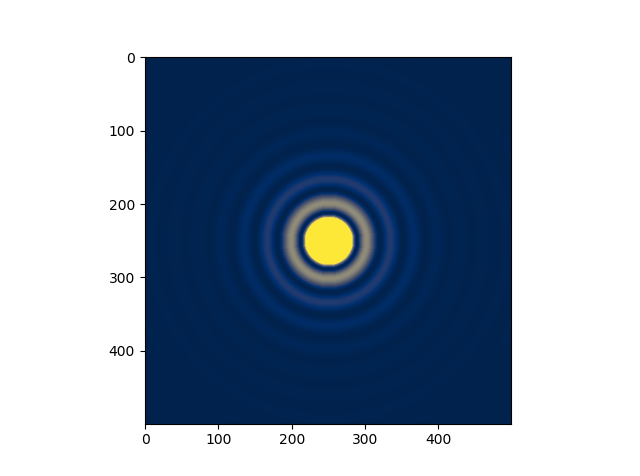
\includegraphics[width=0.7\linewidth]{DiffractionPattern}
	\caption{OUTPUT of Listing \ref{lst:L6}}
	\label{fig:diffractionpattern}
\end{figure}
\subsection{Errors on Integrals}
The numerical integrals mentioned before were only approximations. Therefore, we are able to derive their approximation errors to get an idea of the precision involved.\\

We define $x_{k}=a+kh$, a point to evaluate $f(x)$ at. Now Taylor expansion at $x_{k-1} $is given by:
\[ f(x)= f(x_{k-1})+(x-x_{k-1})f^{'}(x_{k-1})+\dfrac{1}{2!}(x-x_{k-1})^{2}f^{"}(x_{k-1}) + ... \]
\par Integrating $f(x)$ in range $[x_{k-1},x_{k}]$ gives:
\[ \int_{x_{k-1}}^{x_{k}}f(x)\cdot dx = f(x_{k-1})\int_{x_{k-1}}^{x_{k}}dx + f^{'}(x_{k-1})\int_{x_{k-1}}^{x_{k}}(x-x_{k-1})\cdot dx +\dfrac{f^{"}(x_{k-1})}{2}\int_{x_{k-1}}^{x_{k}}(x-x_{k-1})^{2}\cdot dx + ....
\]
\par Substituting $u=x-x_{k-1}$ :
\[ \begin{split}
\int_{x_{k-1}}^{x_k} f(x)\cdot dx&=f(x_{k-1})\int_{0}^{h}du+f^{'}(x_{k-1})\int_{0}^{h}u\cdot du + \dfrac{f^{"}(x_{k-1})}{2}\int_{0}^{h}u^{2}\cdot du+ ....\\
&=hf(x_{k-1})+\dfrac{h^{2}}{2}f^{'}(x_{k-1})+\dfrac{h^{3}}{6}f^{"}(x_{k-1})+O(h^{4})\\
\end{split} \]
\par where,  $O(h^{4})$ denotes the rest of the terms in the series, those in $h^{4}$ and higher.\\
\par We can do similar expansion around $x=x_{k}$ and again integrate within the given range. Taking the average of the integrals in range $[x_{k-1},x_{k}]$ with Taylor expansions at both $x_{k-1} and x_{k}$ gives us:
\[\int_{x_{k-1}}^{x_{k}}f(x)\cdot dx = \dfrac{h}{2}[f(x_{k-1})+f(x_k)]+\dfrac{h^2}{4}[f^{'}(x_{k-1})-f^{'}(x_k)]+\dfrac{h^3}{12}[f^{"}(x_{k-1})+f^{"}(x_k)]+O(h^4)
\]
\par Finally, we sum this expression over all slices $k$ to get the full integral that we want:
\[\begin{split}
\int_{a}^{b}f(x)\cdot dx& =\sum_{k=1}^{N}\int_{x_{k-1}}^{x_{k}}f(x)dx\\
&=\dfrac{h}{2}\sum_{k=1}^{N}[f(x_{k-1})+f(x_{k})]+\dfrac{h^{2}}{4}[f^{'}(a)-f^{'}(b)]+\dfrac{h^{3}}{12}\sum_{k=1}^{N}[f^{"}(x_{k-1})+f^{"}(x_{k})]+O(h^{4})\\
\end{split}
\]
\par Making the changes necessary to fit the above equation to the \textbf{Trapezoidal Rule} we have:
\[\int_{a}^{b}f(x)\cdot dx = \dfrac{h}{2}\sum_{k=1}^{N}[f(x_{k-1})+f(x_{k})]+\dfrac{h^{2}}{12}[f^{'}(a)-f^{'}(b)] +O(h^{4})
\]
Thus, to leading order in h, the value of the terms dropped when we use the trapezoidal rule, which equals the approximation error $\epsilon$ on the integral is:
\[ \epsilon=\dfrac{h^{2}}{12}[f^{'}(a)-f^{'}(b)]\]
This is the \textit{Euler-Maclaurin formula} for the error on the trapezoidal rule. Similar operations for the \textbf{Simpson's Rule} yield:
\[ \epsilon=\dfrac{h^{4}}{90}[f^{\prime\prime\prime}(a)-f^{\prime\prime\prime}(b)] \]
For programming purposes, we use the numerical approach of calculating $\epsilon$ which is given as follows:
\[\begin{split}
\textbf{Trapezoidal Rule }&: \epsilon=\dfrac{1}{3}[I_{2}-I_{1}] \\
\textbf{Simpson's Rule }&: \epsilon=\dfrac{1}{15}[I_{2}-I_{1}]
 \end{split}
 \]

\subsection{Adaptive Integral Method}
\label{subsec:3.4}
This method utilises the numerical approach of calculating the errors. We begin by calculating an approximate integral $I_{1}$ with $N$ steps. Similarly $I_{2}$ is calculated with $2N$ steps. Then, the error will be given by:$$\epsilon=\dfrac{1}{3}[I_{2}-I_{1}]$$ Furthermore, If $\epsilon>\epsilon_{0}$, where $\epsilon_{0}$ is the degree of accuracy, we double the number of steps until $\epsilon<\epsilon_{0}$. This is implemented for the \textbf{Trapezoidal Rule} as follows:
\begin{lstlisting}[language=Python, caption=Adaptive Rule, frame=single, label={lst:L7} ]
def f(x):
	return #Function here
a= #Start Range
b= #End Range
thresh= #threshold
error=1 #Seed Error
N=1 #Repetitions
I1=(f(a)+f(b))/2
while error>thresh:
	N=2*N
	h=(b-a)/N
	s=1/2*(f(a)+f(b))
	for i in range(1,N):
		s+=f(a+i*h)
	I2=h*s
	error=abs(1/3*(I2-I1))
	I1=I2
print(f'The value of integral is {I1} with error {error}')
\end{lstlisting}
\newpage
\subsection{Romberg Integration}





